\documentclass{mwrep}

% Polskie znaki
\usepackage{polski}
\usepackage[utf8]{inputenc}
\usepackage[T1]{fontenc}
\usepackage{lmodern}
\usepackage{indentfirst}

% Strona tytułowa
\usepackage{pgfplots}
\usepackage{siunitx}
\usepackage{paracol}

% Pływające obrazki
\usepackage{float}
\usepackage{svg}
\usepackage{graphicx}

% table of contents refs
\usepackage{hyperref}
\usepackage{cleveref}
\usepackage{booktabs}
\usepackage{listings}


\SendSettingsToPgf
\title{\bf Projekt układu sterowania stanowiska INTECO TCRANE \vskip 0.1cm}
\author{Krystian Guliński \\ Jakub Sikora \\ Konrad Winnicki }
\date{\today}
\pgfplotsset{compat=1.15}	
\begin{document}

\makeatletter
\renewcommand{\maketitle}{\begin{titlepage}
		\begin{center}{
				\LARGE {\bf Politechnika Warszawska}}\\
            \vspace{0.4cm}
            \leftskip-0.9cm
            {\LARGE {\bf \mbox{Wydział Elektroniki i Technik Informacyjnych}}}\\
            \vspace{0.2cm}
            {\LARGE {\bf \mbox{Instytut Automatyki i Informatyki Stosowanej}}}\\
            
            \vspace{5cm}
            \leftskip-1.5cm
			{\bf \Huge \mbox{Systemy automatyki DCS i SCADA} \vskip 0.1cm}
		\end{center}
		\vspace{0.1cm}

		\begin{center}
			{\bf \LARGE \@title}
		\end{center}

		\vspace{10cm}
		\begin{paracol}{2}
			\addtocontents{toc}{\protect\setcounter{tocdepth}{1}}
			\subsection*{Zdający:}
			\bf{ \Large{ \noindent\@author \par}}
			\addtocontents{toc}{\protect\setcounter{tocdepth}{2}}

			\switchcolumn \addtocontents{toc}{\protect\setcounter{tocdepth}{1}}
			\subsection*{Prowadzący:}
			\bf{\Large{\noindent mgr. inż. Andrzej \\ Wojtulewicz}}
			\addtocontents{toc}{\protect\setcounter{tocdepth}{2}}

		\end{paracol}
		\vspace*{\stretch{6}}
		\begin{center}
			\bf{\large{Warszawa, \@date\vskip 0.1cm}}
		\end{center}
	\end{titlepage}
}
\makeatother
\maketitle

\tableofcontents


\chapter{Opis stanowiska}
\label{Opis}

\section{Stanowisko TCRANE}
\label{Opis::TCRANE}
Trójwymiarowy model laboratoryjnego modelu dźwigu ilustruje strukturę współczesnego 
żurawia, skutecznie odwzorowuje stosunek wielkości do maksymalnego podnoszonego 
ładunku. Obiekt jest wielowejściowym i wielowyjściowym systemem wyposażonym w dedykowane
czujniki do mierzenia przemieszczeń i kątów.\\
\indent Stanowisko laboratoryjne T-Crane posiada 5 enkoderów inkrementalnych. Trzy z nich
mierzą położenie elementów napędzanych przez silniki. Dwa z nich znajdują się na karetce
dźwigu i przedstawiają aktualne wychylenie obciążenia od pionu.

\begin{figure}[H]
    \label{Opis::TCRANE::Stanowisko}
    \centering
    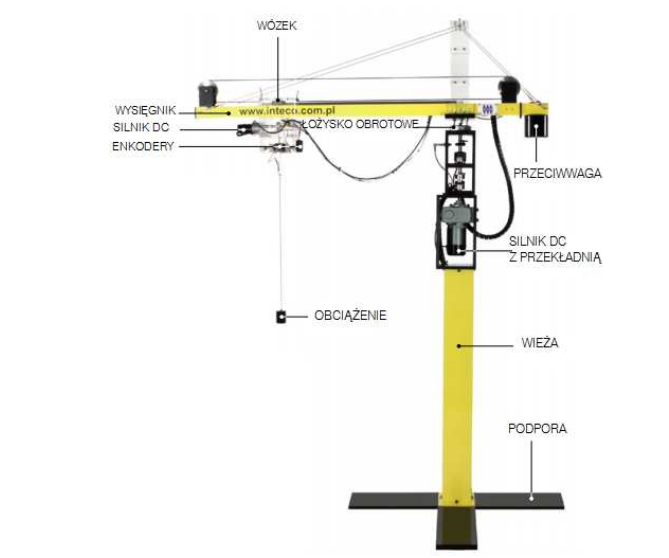
\includegraphics[scale=0.5]{tcrane.png}
    \caption{Stanowisko laboratoryjne TCRANE}
\end{figure}

W ramach projektu laboratoryjnego, mieliśmy wysterować ramię dźwigu w dwóch płaszczyznach:

\begin{itemize}
    \item obrót kolumny dźwigu (wieży)
    \item ruch wózka wzdłuż ramienia
\end{itemize}

\section{Enkodery inkrementalne}
\label{Opis::Enkodery}
Enkoder (przetwornik położenia) służy do pomiaru położenia. W powyższej wersji
mamy do czynienia z przetwornikiem obrotowym. Zatem możemy dzięki niemu określić
położenie kątowe wokół osi. Jeżeli podłączymy go do liniowego układu przeniesienia napędu
możemy określić położenie liniowe wyrażane w odległości.\\
\indent Do określenia kierunku potrzebujemy dwóch sygnałów (tzw.
fazy A i B).Do określenia pozycji wykorzystujemy dwa wejścia do zliczania 
impulsów z fazy A i B. Wykrywanie kierunku jest wykonywane
automatycznie w sterowniku. Przy pomocy mechanizmu sprzętowych liczników możemy w
dowolnym momencie odczytać aktualne położenie enkodera. W pamięci
sterownika pozycja będzie przedstawiona w odpowiednim rejestrze 32 bitowym.\\
\indent Zliczanie impulsów odbywa się za pomocą liczników \emph{High Speed Counter}.
Pozycja zadawana w procentach jest programowo zamieniana na impulsy enkodera 
według następującego wzoru:

$$ I = \frac{STPT * MAX}{100\%}$$

Dla wózka jeżdżącego wzdłuż ramienia $$MAX_{wozek} = 9000,$$
natomiast dla wieży $$MAX_{wieza} = 2300$$

\section{Opis wejść i wyjść obiektu}
\label{Opis::IO}

\subsection{Wejścia cyfrowe}
\label{Opis::IO::Input}

\begin{table}[H]
    \centering
    \begin{tabular}{|p{0.1\linewidth}|p{0.6\linewidth}|}
	\hline
	Wejście & Opis \\ \hline
	X0 & Enkoder inkrementalny, fala A, oś X              \\ \hline
	X1 & Enkoder inkrementalny, fala B, oś X                   \\ \hline
	X2 & Enkoder inkrementalny, fala A, oś Y 		         \\  \hline
	X3 & Enkoder inkrementalny, fala B, oś Y            \\ \hline
	X4 & Enkoder inkrementalny, fala A, oś AX 		         \\  \hline
    X5 & Enkoder inkrementalny, fala B, oś AX           \\ \hline
    X6 & Enkoder inkrementalny, fala A, oś AY 		         \\  \hline
    X7 & Enkoder inkrementalny, fala B, oś AY            \\ \hline
    X10 & Enkoder inkrementalny, fala A, oś Z  		         \\  \hline
    X11 & Enkoder inkrementalny, fala B, oś Z            \\ \hline
    X12 & Wyłącznik krańcowy, oś Z 		         \\  \hline
    X13 & Wyłącznik krańcowy, oś X 		         \\  \hline
    X14 & Wyłącznik krańcowy, oś Y 		         \\  \hline
    X15 & Flaga limitu temperatury, oś Z 		         \\  \hline
    X16 & Flaga limitu temperatury, oś Y 		         \\  \hline
    X17 & Flaga limitu temperatury, oś X 		         \\  \hline
	\end{tabular}
    \caption{Wejścia instalacji INTECO TCRANE}
\end{table}
\newpage

\subsection{Wyjścia cyfrowe}
\label{Opis::IO::Output}

\begin{table}[H]
    \centering
    \begin{tabular}{|p{0.1\linewidth}|p{0.6\linewidth}|}
	\hline
    Wejście & Opis \\ \hline
    Y0 & Sygnał PWM dla silnika DC, oś X  \\  \hline
	Y1 & Sygnał PWM dla silnika DC, oś Z  \\ \hline
	Y2 & Sygnał PWM dla silnika DC, oś Y  \\ \hline
	Y3 & Hamulec silnika DC, oś Z 		  \\  \hline
	Y4 & Wybór kierunku obrotów silnika DC, oś Z         \\ \hline
	Y5 & Hamulec silnika DC, oś Y 		  \\  \hline
	Y6 & Wybór kierunku obrotów silnika DC, oś Y         \\ \hline
    Y7 & Hamulec silnika DC, oś X 		  \\  \hline
    Y10 & Wybór kierunku obrotów silnika DC, oś X         \\ \hline
	\end{tabular}
	\caption{Wyjścia instalacji INTECO TCRANE}
\end{table}

\chapter{Sterownik PLC}
\label{PLC}

\section{Konfiguracja sprzętowa}
\label{PLC::Konfiguracja}

\subsection{Ethernet}
\label{PLC::Konfiguracja::Ethernet}

W celu umożliwienia komunikacji sterownika z komputerem PC, odpowiednio skonfigurowaliśmy
połączenie w sieci Ethernet. Komunikacja odbywa się za pomocą protokołu SLMP (SeamLess 
Message Protocol) na porcie 1280. 

\begin{figure}[H]
    \label{PLC::Konfiguracja::Ethernet::Window}
    \centering
    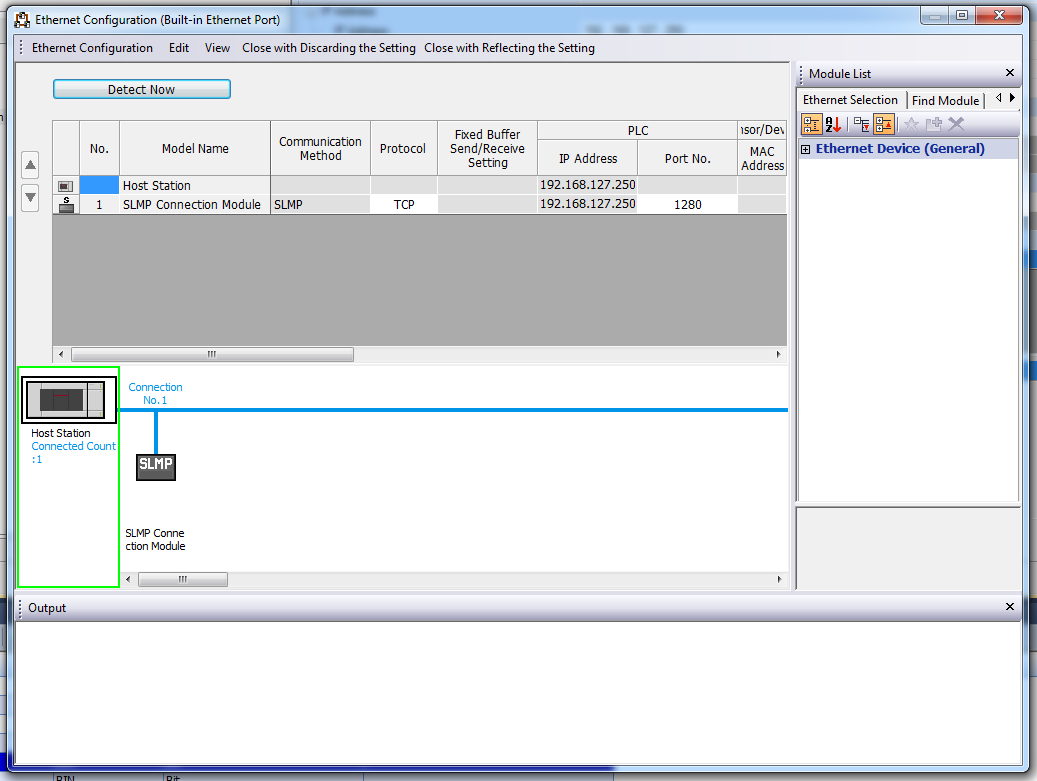
\includegraphics[scale=0.3]{ethernet.png}
    \caption{Konfiguracja komunikacji w sieci Ethernet w systemie GX Works3}
\end{figure}

\subsection{Analog}
\label{PLC::Konfiguracja::Analog}

Obsługa wejść analogowych została przedstawiona jako jedno z kryterium oceny projektu.
Niestety, stanowisko INTECO TCRANE nie zawiera żadnych wejść i wyjść analogowych. 

\subsection{High Speed Counter}
\label{PLC::Konfiguracja::HIOEN}

Odczyt z enkoderów inkrementalnych odbywał się za pomocą specjalnych liczników \emph{High Speed
Counter}. Skonfigurowaliśmy dwa kanały CH1 oraz CH5 do odczytu pozycji wózka oraz obrotu wieży. 
Wartość pozycji wózka odczytywaliśmy spod adresu \texttt{SD4500} a wartość pozycji kątowej wieży 
spod adresu \texttt{SD4620}.

\newpage

\begin{figure}[H]
    \label{PLC::Konfiguracja::HIOEN::WindowCH1}
    \centering
    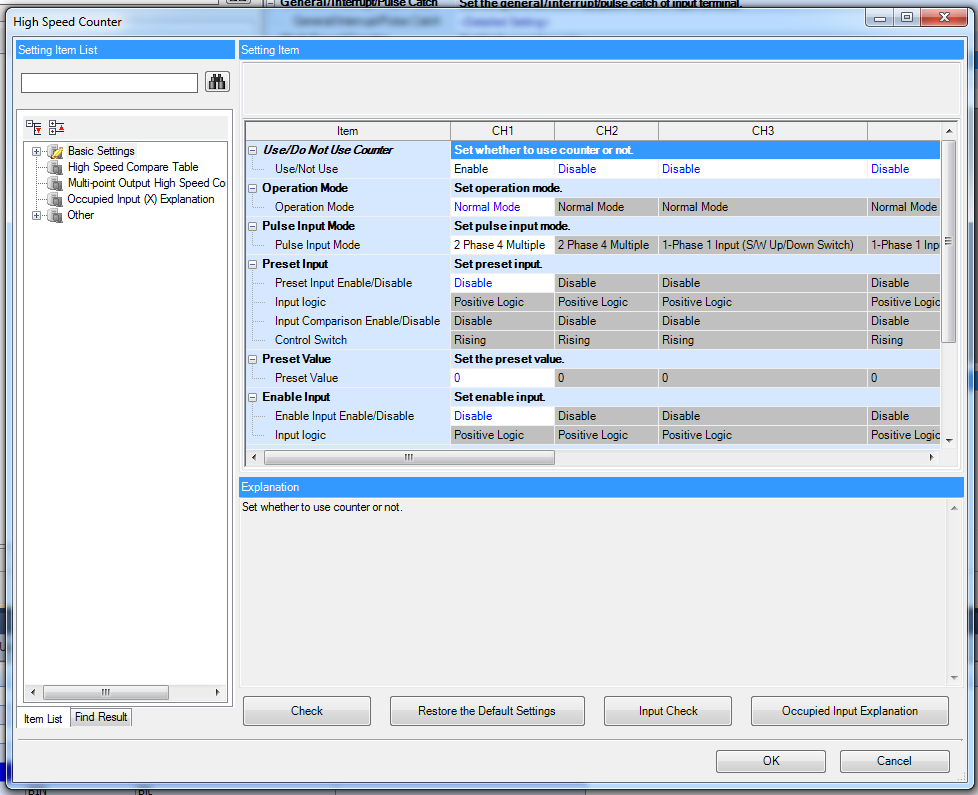
\includegraphics[scale=0.3]{hioen.png}
    \caption{Okno konfiguracji kanału \emph{CH1} High Speed Counters w systemie GX Works3}
\end{figure}

\begin{figure}[H]
    \label{PLC::Konfiguracja::HIOEN::WindowCH5}
    \leftskip-1.5cm
    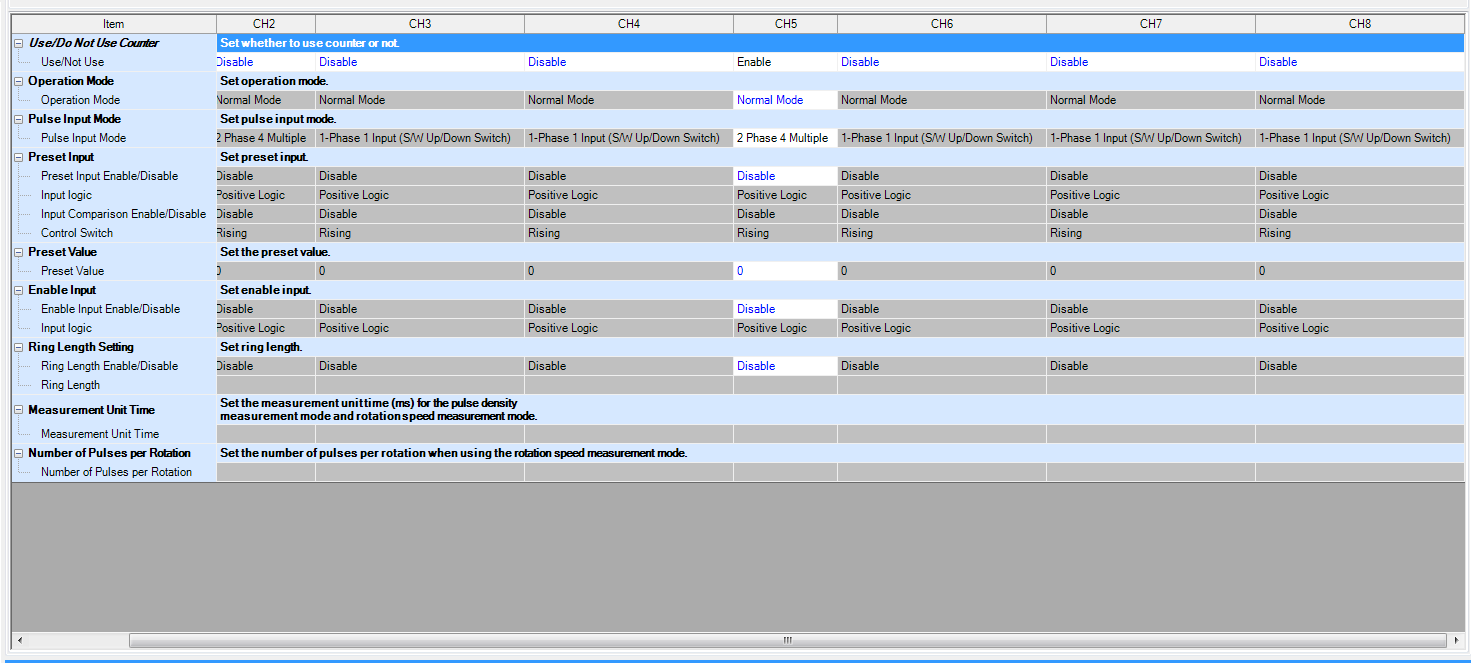
\includegraphics[scale=0.3]{hioen2.png}
    \caption{Okno konfiguracji kanału \emph{CH5} High Speed Counters w systemie GX Works3}
\end{figure}


\subsection{Wyjścia PWM}
\label{PLC::Konfiguracja::PWM}
Wyjścia analogowe zostały zastąpione wyjściami cyfrowymi PWM. PWM czyli \emph{Pulse Width Modifiaction} to 
technika przybliżania sygnału analogowego poprzez sygnał prostokątny o zmiennym wypełnieniu. W projekcie,
w ten sposób sterowaliśmy silnikami prądu stałego obiektu. W programie GX Works3 odpowiednio
skonfigurowaliśmy 3 kanały PWM do współpracy z trzema silnikami obiektu. Do dalszej pracy 
wykorzystaliśmy tylko dwa z nich. Kanał \emph{CH1} służył do sterowania wyciągnikiem, kanał \emph{CH2}
sterował silnikiem wózka a kanał \emph{CH3} zajmował się sterowaniem silnika obracającym wieżą.




\begin{figure}[H]
    \label{PLC::Konfiguracja::HIOEN::WindowCH5}
    \centering
    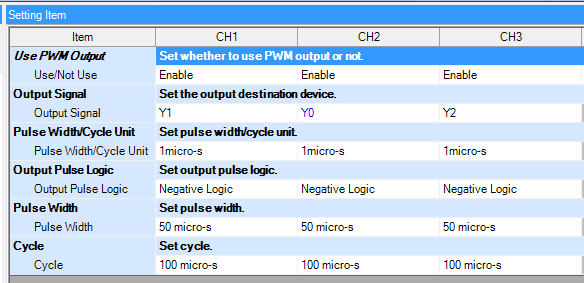
\includegraphics[scale=0.5]{pwm.png}
    \caption{Okno konfiguracji kanałów PWM w systemie GX Works3}
\end{figure}

\section{Mechanizm labeli}
\label{PLC::Labels}

Zarejestrowaliśmy szereg labeli globalnych zastępujących m.in. wejścia X, ponieważ własne nazwy zwiększają uniwersalność i znacznie zwiększają czytelność kodu.

\begin{figure}[H]
    \label{PLC::Konfiguracja::HIOEN::WindowCH5}
    \centering
    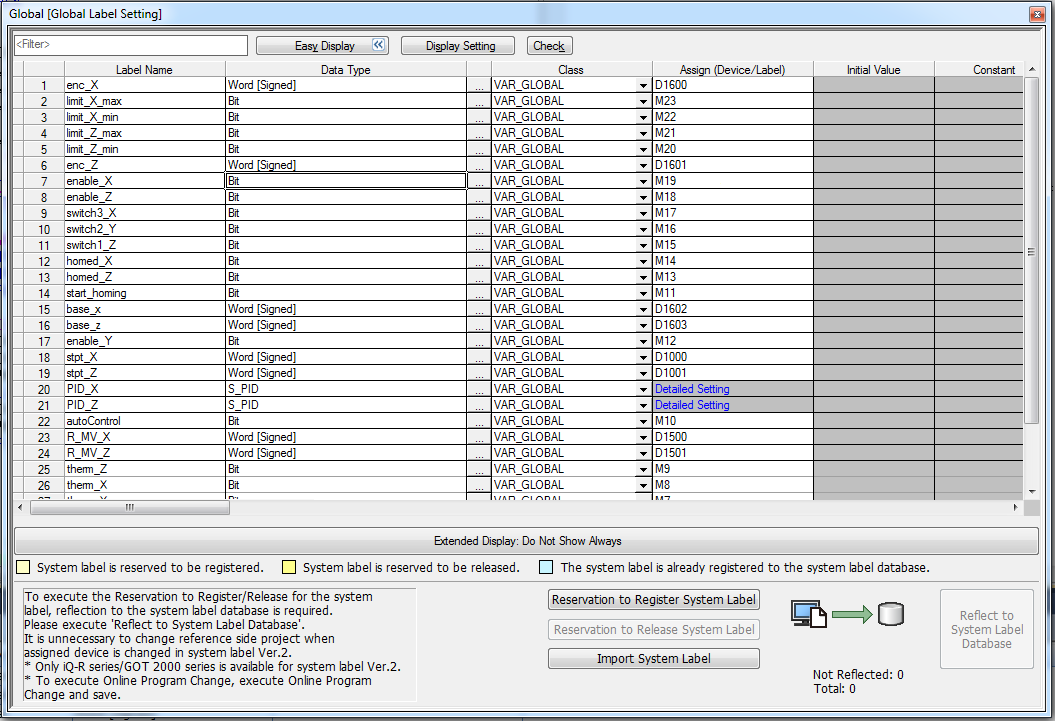
\includegraphics[scale=0.5]{global_label.png}
    \caption{Ustawienia labeli globalnych}
\end{figure}

\section{Skalowanie i bazowanie}
\label{PLC::Bazowanie}

\subsection{Skalowanie osi X}
	Odczytując wartości enkodera osi X w dwóch skrajnych pozycjach i dzieląc ich różnicę(9421) przez maksymalną założoną wartość pozycji zadanej(100) otrzymaliśmy zaokrąglony współczynnik skalowania(94)
 Efektem jest operacja:
MOV(TRUE, stpt\_X*K94, PID\_X.SV);

\subsection{Skalowanie osi Z}
	Odczytując wartości enkodera osi Z w dwóch skrajnych pozycjach i dzieląc ich różnicę(2300) przez maksymalną założoną wartość pozycji zadanej(100) otrzymaliśmy zaokrąglony współczynnik skalowania(23)
 Efektem jest operacja:
MOV(TRUE, stpt\_Z*K23, PID\_Z.SV);

\subsection{Bazowanie osi}
Bazowanie wszystkich osi inicjowane jest stanem wysokim zmiennej start\_homing. Po spełnieniu tego warunku rozpoczynany jest ruch osi w kierunku krańcówek. Osie poruszają się do chwili gdy osiągnął pozycje swoich krańcówek bazujących. W następnym kroku osie są zatrzymywane, ustawiane są bity informujące o zakończeniu bazowania konkretnej osi i wykonywane jest zerowanie liczników enkoderów osi.
Zbazowanie każdej z osi kończy proces bazowania dzwigu. Możliwe staje się sterowanie za pomocą pozycji zadanych poprzez regulatory PID.



IF start\_homing = TRUE THEN
	
\quad IF homed\_X = FALSE THEN
		
\quad \quad IF switch3\_X = FALSE THEN

\quad \quad \quad Y7:=TRUE; // DEAKTYWACJA HAMULCA

\quad \quad \quad PWM(TRUE, K30, K100, Y0); // PWM OSI X - KARETKA

\quad \quad \quad ELSE

\quad \quad \quad PWM(FALSE, K1, K100, Y0);

\quad \quad \quad Y7:=FALSE; // AKTYWACJA HAMULCA

\quad \quad \quad DHCMOVP(TRUE, 0, 0, SD4500); // WYZEROWANIE ENKODERA OSI X

\quad \quad \quad homed\_X:=TRUE;

\quad \quad END\_IF;

\quad END\_IF;

\quad IF homed\_Z = FALSE THEN

\quad \quad IF switch1\_Z = FALSE THEN

\quad \quad \quad Y5:=TRUE; // DEAKTYWACJA HAMULCA

\quad \quad \quad PWM(TRUE, K30, K100, Y2); // PWM OSI Z - OBRÓT DZWIGU

\quad \quad \quad ELSE

\quad \quad \quad PWM(FALSE, K1, K100, Y2);

\quad \quad \quad DHCMOVP(TRUE, 0, 0, SD4620); // WYZEROWANIE ENKODERA OSI Z

\quad \quad \quad Y5:=FALSE; // AKTYWACJA HAMULCA

\quad \quad \quad homed\_Z:=TRUE;

\quad \quad END\_IF;

\quad END\_IF;
		
\quad IF homed\_X AND homed\_Z THEN

\quad \quad start\_homing := FALSE;

\quad END\_IF;

END\_IF;


\section{Obsługa I/O cyfrowych}
\label{PLC::IOCyfrowe}

\subsection{Odczyt wejść cyfrowych}
Stany wejść cyfrowych w celu zwiększenia czytelności kodu są przepisywane do uprzednio zdefiniowanych labeli, które następnie są wykorzystywane w programie.
	
Przykładowy odczyt stanu krańcówek osi:
	
MOVB(TRUE, X13, switch3\_X);

MOVB(TRUE, X14, switch2\_Y);

MOVB(TRUE, X12, switch1\_Z);



Dalsze przykładowe wykorzystanie labeli do sterowania:

IF switch3\_X = FALSE THEN

\quad Y7:=TRUE; // DEAKTYWACJA HAMULCA

\quad PWM(TRUE, K30, K100, Y0); // PWM OSI X - KARETKA

\quad ELSE

\quad PWM(FALSE, K1, K100, Y0);

\quad Y7:=FALSE; // AKTYWACJA HAMULCA

\quad DHCMOVP(TRUE, 0, 0, SD4500); // WYZEROWANIE ENKODERA OSI X

\quad homed\_X:=TRUE;

END\_IF;
 
\subsection{Zapis wyjść cyfrowych}
Zapis wyjść cyfrowych odbywa się poprzez bezpośrednie przypisanie stanu wyjścia. Nie zdecydowaliśmy się na zastosowanie dedykowanych labeli, ponieważ wyjść było stosunkowo niewiele.
	Przykładowy zapis wyjścia cyfrowego:
		Y5:=TRUE; // DEAKTYWACJA HAMULCA OSI Z


\section{PID}
\label{PLC::PID}

Zastosowaliśmy wbudowaną strukturę regulatora PID. Do jej wykorzystania potrzebne było stworzenie struktury S\_PID zawierającej SV, PV, MV, parametry regulatora oraz bit aktywujący regulator.

\begin{figure}[H]
    \label{PLC::Konfiguracja::HIOEN::WindowCH5}
    \centering
    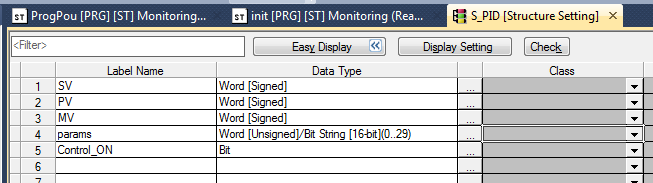
\includegraphics[scale=0.5]{s_pid_struct.png}
    \caption{Struktura S\_PID}
\end{figure}


W programie inicjującym znajduje się inicjalizacja parametrów regulatorów PID 

//Parametry regulatora wbudowanego PID osi X

PID\_X.params[0] := K100; //okres regulacji w milisekundach

PID\_X.params[3] := K3; //wzmocnienie regulatora P

PID\_X.params[4] := K5; //TI = 0 oznacza nieskonczony czas calkowania - inaczej

//mowiac calkowanie wylaczone

PID\_X.params[5] := K0; //KD = 0 oznacza zerowe wzmocnienie rozniczkowania

PID\_X.params[6] := K0; //TD = 0 oznacza wylaczone rozniczkowanie 

PID\_X.params[22] := K100; //gorny limit wartosci wyjsciowej z regulatora - zapobiega

//rowniez efektowi wind-up

PID\_X.params[23] := K1; //dolny limit wartosci wyjsciowej z regulatora - -||-

SET(TRUE, PID\_X.params[1].5); //aktywacja limitow na wyjsciu regulatora

SET(TRUE, PID\_X.params[1].0); //trzeba odwrocic kierunek dzialania PID 


//Parametry regulatora wbudowanego PID osi Z

PID\_Z.params[0] := K100; //okres regulacji w milisekundach

PID\_Z.params[3] := K1; //wzmocnienie regulatora P

PID\_Z.params[4] := K2; //TI = 0 oznacza nieskonczony czas calkowania - inaczej

//mowiac calkowanie wylaczone

PID\_Z.params[5] := K0; //KD = 0 oznacza zerowe wzmocnienie rozniczkowania

PID\_Z.params[6] := K0; //TD = 0 oznacza wylaczone rozniczkowanie 

PID\_Z.params[22] := K100; //gorny limit wartosci wyjsciowej z regulatora - zapobiega

//rowniez efektowi wind-up

PID\_Z.params[23] := K0; //dolny limit wartosci wyjsciowej z regulatora - -||-

SET(TRUE, PID\_Z.params[1].5); //aktywacja limitow na wyjsciu regulatora

SET(TRUE, PID\_Z.params[1].0); //trzeba odwrocic kierunek dzialania PID 


Regulatory PID pracują w głównym programie. Kolejne wartości sterowania MV wyznaczane są poprzez wywołania funkcji PID(). Jeśli wyznaczone MV jest większe od 50 wykonywany jest ruch w przód z zadanym wypełnieniem PWM, a w przeciwnym wypadku wykonywany jest ruch w tył z zadanym wypełnieniem PWM.

Sekcja regulatora PID osi X:

\quad MOVB(TRUE, TRUE, PID\_X.Control\_ON);

\quad MOV(TRUE, enc\_X, PID\_X.PV);

\quad MOV(TRUE, stpt\_X*K94, PID\_X.SV);

\quad PID(PID\_X.Control\_ON, PID\_X.SV , PID\_X.PV , PID\_X.params[0] , PID\_X.MV); 

\quad PWM(TRUE, PID\_X.MV, K100, Y0); // PWM OSI X - KARETKA				
	
\quad IF PID\_X.MV < K50 THEN

\quad \quad MOVB(TRUE, FALSE, Y10);

\quad \quad MOVB(TRUE, TRUE, Y7);

\quad \quad PWM(TRUE, K51-PID\_X.MV, K100, Y0); // PWM OSI X - KARETKA		
	
\quad ELSE 

\quad \quad IF PID\_X.MV > K50 THEN

\quad \quad \quad MOVB(TRUE, TRUE, Y10);

\quad \quad \quad MOVB(TRUE, TRUE, Y7);

\quad \quad \quad PWM(TRUE, PID\_X.MV-K49, K100, Y0); // PWM OSI X - KARETKA	
	
\quad \quad \quad ELSE	

\quad \quad \quad MOVB(TRUE, FALSE, Y7);

\quad \quad \quad PWM(FALSE, K1, K100, Y0); // PWM OSI X - KARETKA	

\quad \quad END\_IF;

\quad END\_IF;

Sekcja regulatora PID osi Z:

\quad MOVB(TRUE, TRUE, PID\_Z.Control\_ON);

\quad MOV(TRUE, enc\_Z, PID\_Z.PV);

\quad MOV(TRUE, stpt\_Z*K23, PID\_Z.SV);

\quad PID(PID\_Z.Control\_ON, PID\_Z.SV , PID\_Z.PV , PID\_Z.params[0] , PID\_Z.MV); 

\quad PWM(TRUE, PID\_Z.MV, K100, Y2); // PWM OSI Z - OBRÓT DZWIGU				
	
\quad IF PID\_Z.MV < K50 THEN

\quad \quad MOVB(TRUE, FALSE, Y6);

\quad \quad MOVB(TRUE, TRUE, Y5);

\quad \quad PWM(TRUE, K51-PID\_Z.MV, K100, Y2); // PWM OSI Z - OBRÓT DZWIGU			

\quad \quad ELSE 

\quad \quad IF PID\_Z.MV > K50 THEN

\quad \quad \quad MOVB(TRUE, TRUE, Y6);

\quad \quad \quad MOVB(TRUE, TRUE, Y5);

\quad \quad \quad PWM(TRUE, PID\_Z.MV-K49, K100, Y2); // PWM OSI Z - OBRÓT DZWIGU		

\quad \quad \quad ELSE	

\quad \quad \quad MOVB(TRUE, FALSE, Y5);

\quad \quad \quad PWM(FALSE, K1, K100, Y2); // PWM OSI Z - OBRÓT DZWIGU	

\quad \quad END\_IF;

\quad END\_IF;




\section{Tryb sterowania ręcznego}
\label{PLC::Reka}

Sterowanie ręczne możliwe jest po zresetowaniu flagi AUTO\_CONTROL(flaga domyślnie ustawiona). Jeśli flaga jest zresetowana program przechodzi do sekcji kodu w której odbywa się bezpośrednie wysterowanie wyjść PWM wartościami zmiennych R\_MV\_Z dla osi Z i R\_MV\_X dla osi X
sekcja kodu sterowania ręcznego osią Z:

\quad IF enc\_Z > K2350 OR enc\_Z < -K50 THEN

\quad \quad // PRZEKROCZENIE ZAKRESÓW OSI Z

\quad \quad MOVB(TRUE, FALSE, Y5);

\quad \quad PWM(FALSE, K1, K100, Y2); // PWM OSI Z - OBRÓT DZWIGU

\quad \quad MOVB(TRUE, FALSE, homed\_Z);

\quad \quad ELSE

\quad \quad //STEROWANIE RĘCZNE OSI Z

\quad \quad PWM(TRUE, R\_MV\_Z, K100, Y2);	// PWM OSI Z - OBRÓT DZWIGU

\quad \quad IF R\_MV\_Z < K50 THEN

\quad \quad \quad MOVB(TRUE, FALSE, Y6);

\quad \quad \quad MOVB(TRUE, TRUE, Y5);

\quad \quad \quad PWM(TRUE, K51-R\_MV\_Z, K100, Y2); 	// PWM OSI Z - OBRÓT DZWIGU	

\quad \quad \quad ELSE 

\quad \quad \quad IF R\_MV\_Z > K50 THEN

\quad \quad \quad \quad MOVB(TRUE, TRUE, Y6);

\quad \quad \quad \quad MOVB(TRUE, TRUE, Y5);

\quad \quad \quad \quad PWM(TRUE, R\_MV\_Z-K49, K100, Y2); // PWM OSI Z - OBRÓT DZWIGU

\quad \quad \quad \quad ELSE

\quad \quad \quad \quad MOVB(TRUE, FALSE, Y5);

\quad \quad \quad \quad PWM(FALSE, K1, K100, Y2); 

\quad \quad \quad END\_IF;

\quad \quad END\_IF;

\quad END\_IF;

sekcja kodu sterowania ręcznego osią X:

\quad IF enc\_X > K9450 OR enc\_X < -K50 THEN

\quad \quad // PRZEKROCZENIE ZAKRESÓW OSI X

\quad \quad MOVB(TRUE, FALSE, Y7);

\quad \quad PWM(FALSE, K1, K100, Y0); // PWM OSI X - KARETKA

\quad \quad MOVB(TRUE, FALSE, homed\_X);

\quad \quad ELSE\quad 

\quad \quad // STEROWANIE RĘCZNE OSI X\quad 

\quad \quad PWM(TRUE, R\_MV\_X, K100, Y0); // PWM OSI X - KARETKA\quad \quad 

\quad \quad \quad 

\quad \quad IF R\_MV\_X < K50 THEN

\quad \quad MOVB(TRUE, FALSE, Y10);

\quad \quad \quad MOVB(TRUE, TRUE, Y7);

\quad \quad \quad PWM(TRUE, K51-R\_MV\_X, K100, Y0); // PWM OSI X - KARETKA\quad \quad 

\quad \quad \quad ELSE 

\quad \quad \quad IF R\_MV\_X > K50 THEN

\quad \quad \quad \quad MOVB(TRUE, TRUE, Y10);

\quad \quad \quad \quad MOVB(TRUE, TRUE, Y7);

\quad \quad \quad \quad PWM(TRUE, R\_MV\_X-K49, K100, Y0); // PWM OSI X - KARETKA\quad 

\quad \quad \quad \quad ELSE\quad 

\quad \quad \quad \quad MOVB(TRUE, FALSE, Y7);

\quad \quad \quad \quad PWM(FALSE, K1, K100, Y0); // PWM OSI X - KARETKA\quad 

\quad \quad \quad END\_IF;

\quad \quad END\_IF;

\quad END\_IF;


\section{Zabezpieczenia ruchów krańcowych}
\label{PLC::Krancowki}

W projekcie założyliśmy, że sytuacja w której któraś z osi wyjdzie poza założony dopuszczalny zakres ruchów jest ona natychmiast zatrzymywana i gaszona jest flaga zbazowania danej osi. Działaniem naprawczym w takiej sytuacji jest przejście na tryb sterowania automatycznego i ponowne zainicjowanie bazowania osi ustawiając flagę start\_homing
sekcja kodu zabezpieczająca ruchy krańcowe osi X:

\quad IF homed\_X = TRUE THEN

\quad \quad IF enc\_X > K9450 OR enc\_X < -K50 THEN

\quad \quad \quad MOVB(TRUE, FALSE, Y7);

\quad \quad \quad PWM(FALSE, K1, K100, Y0); // PWM OSI X - KARETKA

\quad \quad \quad MOVB(TRUE, FALSE, homed\_X);

\quad \quad ELSE\quad \quad 

\quad \quad \quad //automatyczne lub ręczne sterowanie osi X

\quad \quad \quad …

\quad \quad END\_IF;

\quad END\_IF;



sekcja kodu zabezpieczająca ruchy krańcowe osi Z:



\quad IF homed\_Z = TRUE THEN

\quad \quad IF enc\_Z > K2350 OR enc\_Z < -K50 THEN

\quad \quad \quad MOVB(TRUE, FALSE, Y5);

\quad \quad \quad PWM(FALSE, K1, K100, Y2); // PWM OSI Z - OBRÓT DZWIGU

\quad \quad \quad MOVB(TRUE, FALSE, homed\_Z);

\quad \quad ELSE\quad 

\quad \quad \quad //automatyczne lub ręczne sterowanie osi Z

\quad \quad \quad …

\quad \quad END\_IF;

\quad END\_IF;



\section{Język ST}
\label{PLC::ST}

Listingi kodu zawarte powyżej jednoznacznie wskazują na pomyślne wykorzystanie języka ST.

\chapter{Realizacja w systemie MAPS}
\label{MAPS}

\section{Panel operatorski}
\label{MAPS::PanelOperatorski}

Na podstawie odpowiednio wykonanej wcześniej konfiguracji sprzętowej sterownika PLC jesteśmy w stanie bezpośrednio połączyć działanie stanowiska z systemem MAPS. Po uruchomieniu serwera (oprogramowania \emph{MAPS Server} i \emph{Agent Server}) i środowiska do projektowania interfejsów operatorskich (\emph{MAPS Designer}) rozpoczęsliśmy od utworzenia projektu.

Kolejnym krokiem jest dodanie do systemu MAPS odpowiednich agentów. Akwizycją danych poprzez uchwyty do agentów zajmuje się \emph{Agent Server}. Aby nasze środowisko graficzne miało dostęp do tych danych należy zdefiniować zbiór agentów dla naszego stanowiska. W zadaniu wykorzystujemy podstawowe rodzaje agentów służące do pozyskiwania danych. 

\begin{figure}[H]
    \label{MAPS::PanelOperatorski}
  
    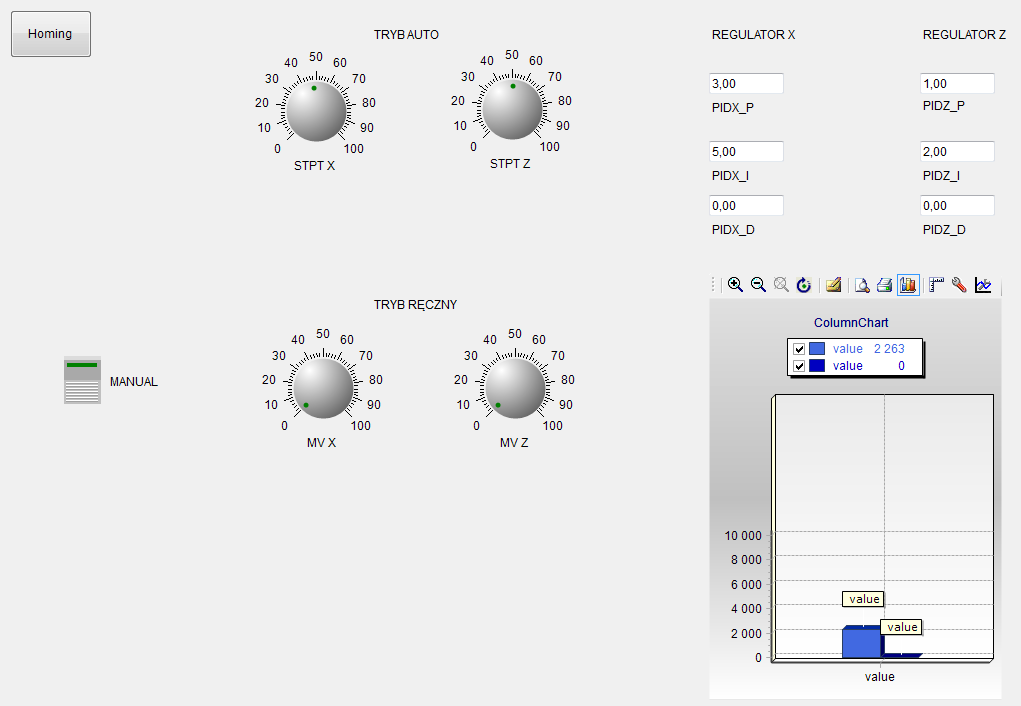
\includegraphics[scale=0.45]{panel_operatorski.png}
    \caption{Panel operatorski stanowiska w systemie MAPS}
\end{figure}

Przy dodawaniu nowych agentów należało zwrócić uwagę na funkcjonalność jaką będziemy chcieli uzyskać. Dane, które będziemy chcieli tylko i wyłącznie wyświetlać nie powinny być oznaczone jako edytowalne z poziomu interfejsu graficznego (pole  \emph{Output enabled}). Zapewnia to większe zabezpieczenie na błędy w trakcie projektowania środowiska graficznego, ponieważ dane wyświetlane mogą być krytyczne z punktu widzenia stanowiska, a ich zewnętrzna zmiana może spowodować awarie. Dane, na które operator będzie mógł wpływać z poziomu środowiska graficznego analogicznie muszą być oznaczone jako edytowalne. Ogólnie przy definiowaniu agentów należy podwójnie sprawdzać poprawność wpisywanych adresów, szczególnie w przypadku struktur, do których trzeba wyznaczać offset od adresu początkowego struktury przy okrelnianiu agenta dla jej pola.

Otrzymany panel operatorski realizuje określoną w zadaniu funkcjonalność, informuje operatora o stanie obiektu oraz pozwala na wpływ na sposób i parametry sterowania obiektem.

\section{Kalibracja}
\label{MAPS::Kalibracja}

Praca z obiektem rozpoczyna się od skalibrowania jego enkoderów absolutnych na podstawie krańcówek umieszczonych na osiach obiektu. Inicjalizacja tego procesu rozpoczyna się od naciśnięcia znajdującego się w lewej górnej części przycisku \emph{Homing}. Po restarcie urządzenia nie jest możliwy żaden tryb pracy bez pomyślnego przejścia przez proces kalibracji, dlatego przycisk umieszczony jest intuicyjnie w lewej górnej części interfejsu w celu określenia odpowiedniej kolejności postępowania w trakcie obsługi obiektu.

\section{Sterowanie auto/ręka}
\label{MAPS::AutoReka}

Sterowanie w trybie automatycznym pozwala na ustawianie wartości docelowych stanu obiektu (stopnia obrotu wieży i wysunięcia wózka). Zmiana tych wartości następuje poprzez ustawienie ich pokrętłem w środowisku graficznym operatora.
Pokrętło \emph{STPT\_Z} odpowiada za wartość zadaną stopnia obrotu wieży w procentach. Pokrętło \emph{STPT\_X} odpowiada natomiast za wartość zadaną stopnia wysunięcia wózka w procentach.

\begin{figure}[H]
    \label{MAPS::PanelOperatorski}
    \centering
    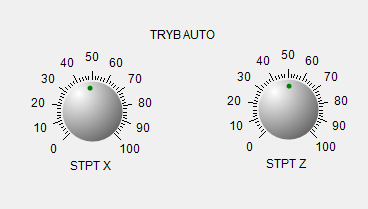
\includegraphics[scale=0.8]{auto.png}
    \caption{Fragment panelu operatorskiego odpowiedzialny za sterowanie w trybie automatycznym}
\end{figure}

Sterowanie w trybie ręcznym jest domyślnie nieaktywne. Aby je aktywować należy wcisnąć przycisk \emph{MANUAL} umieszczony po lewej stronie pokręteł odpowiedzialnych za sterowanie ręczne. Po aktywacji trybu ręcznego mamy możliwość zmiany prędkości obrotu wieży oraz wysunięcia wózka. Pokrętło \emph{MV\_X} odpowiada za zadawanie prędkości wózka, wartości poniżej 50 powodują cofanie się wózka, natomiast wartości powyżej 50 powodu ruch w przód. Pokrętło \emph{MV\_Z} odpowiada za nadawanie prędkości obrototowej wieży, analogicznie wartość poniżej 50 powoduje ruch w lewo, a wartość powyżej 50 powoduje ruch w prawo.

Deaktywacja trybu ręcznego zachodzi poprzez ponowne wciśnięcie przycisku \emph{MANUAL}, po czym następuje przekazanie sterowania do regulatorów w trybie automatycznym.

\begin{figure}[H]
    \label{MAPS::PanelOperatorski}
    \centering
    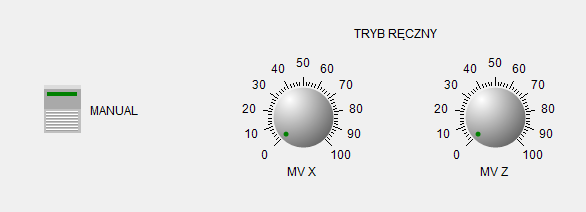
\includegraphics[scale=0.8]{reka.png}
    \caption{Fragment panelu operatorskiego odpowiedzialny za sterowanie w trybie ręcznym}
\end{figure}

\section{Nastawy regulatorów}
\label{MAPS::Nastawy}

Operator w ramach obsługi panelu operatorskiego ma również możliwość zmiany nastaw regulatorów PID odpowiedzialnych za nadążanie za wartościami zadanymi położenia w osiach. Na poniższej ilustracji przedstawiony jest fragment panelu operatorskiego, w którym widoczne są pola tekstowe pozwalające na edycje tych parametrów. Kolumna po lewej stronie pozwala na zmianę parametrów regulatora PID odpowiedzialnego za położenie wózka, natomaist kolumna po prawej stronie pozwala na zmianę parametrów regulatora PID odpowiedzialnego za obrót wieży.

\begin{figure}[H]
    \label{MAPS::PanelOperatorski}
    \centering
    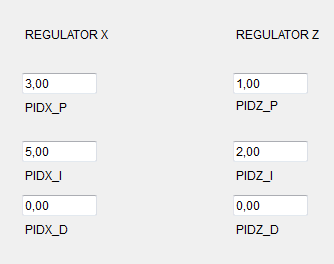
\includegraphics[scale=0.8]{nastawy.png}
    \caption{Fragment panelu operatorskiego odpowiedzialny za zmianę wartości nastaw regulatorów w trybie automatycznym }
\end{figure}


\section{Wykresy}
\label{MAPS::Wykresy}

Znajdujący się na panelu operatora wykres kolumnowy wizualizuje aktualny stan obiektu względem wartości zadanych dla regulatora w celu zapewnienia łatwego sposobu na weryfikacje poprawności stanu obiektu przez operatora nawet z pewnej odległości w sytuacjach opuszczenia stanowiska. 

\end{document}